\documentclass[12pt,fleqn]{article}\usepackage{../../common}
\begin{document}
Ders 16

Bu derste su çarkı denklemlerini hızlıca analiz edeceğiz, ama hemen
ardından onları bırakıp yakından alakalı kaosta herkesin incelediği ama
daha iyi bilinen Lorenz denklem formuna geçeceğiz.

Su çarkı sistemini en son bıraktığımız nokta neydi? Bir mucizeyi
gözlemledik! Sonsuz tane denklem içinden üç tane denklem kaldı, bu üç ODE
geriye kalanlardan tamamen bağımsızdı. Tekrar yazarsak,

$$ \dot{a_1} = \omega b_1 - K a_1 $$

$$ \dot{b_1} = -\omega a_1 + q_1 - Kb_1 $$

$$ \dot{\omega} = \frac{-v\omega}{I} + \frac{\pi gr a_1}{I} $$

$\omega$ çarkın açısal hızıydı, sola ya da sağa ne kadar hızla döndüğünü
temsil ediyordu. $a_1,b_1$ çark etrafındaki su dağılımının ilk harmoniğinin
genlikleri idi [harmonik Fourier açılımındaki ilk $\sin,\cos$ terimlerine
deniyor]. Galiba bizim formülasyona göre $a_1$ $\sin\theta$ için idi, evet
evet, $b_1$ ise $\cos\theta$ içindi. Geri kalanlar sistemi tanımlayan sabit
/ parametreler, $v$ dönme direnci (fren), $K$ suyun akma oranı, $r$
yarıçap, $g$ efektif yerçekim etkisi, $q_1$ giren suyun ilk harmoniği. 

Bu şimdiye kadar gördüğümüz ilk üç boyutlu sistemimiz. Onu analiz etmek
için ne yaparız? İlk refleksimiz herhalde sabit noktalarını bulmaya
uğraşmak. Sonra bu noktalar etrafında lineerizasyon düşünebilirim, aslında
onu bu sistem için yapmayalım, Lorenz sistemi üzerinde yapalım daha
iyi. Ama sabit noktalara bakalım. Bu noktaları bulmak için biraz cebirsel
işlem gerekli, ve bu sabit noktaların bu sistem için ne anlama geldiği
hakkında biraz kafa yormamız gerekli.

$$ 
\dot{a_1} = 0 \implies a_1 = \frac{\omega b_1}{K}  
\mlabel{1} 
$$

$$ 
\dot{b_1} = 0 \implies \omega a_1 = q_1 - K b_1 
\mlabel{2} 
$$

$$ 
\dot{\omega} = 0 \implies a_1 = \frac{v \omega}{\pi gr} 
\mlabel{3}
$$

$a_1,b_1,\omega$'yi bulmak istiyoruz, o zaman üstteki denklemlerde biraz
temizlik, cebirsel manipülasyon yapabiliriz. (1) ve (2)'yi birleştirince
$a_1$'den kurtulabiliriz. (2)'deki $a_1$ için (1)'dekini sokalım ve $b_1$'i
bulalım, sonuç

$$ 
b_1 = \frac{K q_1}{\omega^2 + K^2}  
\mlabel{4} 
$$

$a_1,b_1$ için yıldız kullanabilirdim, $a_1^*,b_1^*$ gibi ama sabit nokta
olduklarını biliyoruz, bunu atlayacağım. (1) ve (3) ile

$$ \frac{\omega b_1}{K} = \frac{v \omega}{\pi gr}$$

Üsttekinin en basit çözümü $w=0$'da çünkü her iki tarafta da bölünende
$\omega$ var. Ama çözüm sıfır değilse diğer çözüm için her iki tarafı
$\omega$ ile böleriz, ve 

$$ 
b_1 = \frac{K v}{\pi gr} 
\mlabel{5} 
$$

elde ederiz. Bu iki durumu biraz düşünelim, $\omega=0$ durumu ne demektir?
Eğer $\omega=0$ ise (1)'e göre $a_1 = 0$, (2)'ye göre $b_1 = q_1 /
K$. $\omega=0$ demek, çark dönmüyor demektir. $a_1=0$ ise içeri akan suyun
sinüssel harmoniği yoktur, tepede simetrik bir dağılım vardır, ve $b_1$'e
göre $q_1$ akış hızı $K$ ile dengelenmiştir, yani su akıyor ve olduğu gibi
dışarı çıkıyor. Başka bir hareket yok. Bu bir sabit nokta, çünkü suyun
dağılımında hiçbir değişim yok, su o yeşil kutucuklar içinde hep aynı
histogram şeklinde duruyor. Diğer parametreler ne olursa olsun bu çözüm her
zaman olası bir çözümdür. Stabil olduğunu söylemiyoruz, ama mevcut olduğunu
söylüyoruz.

$\omega \ne 0$, o zaman 

$$ 
b_1 = \frac{Kv}{\pi gr} = \frac{K q_1}{\omega^2 + K^2} \implies
\omega^2 = \frac{\pi gr q_1}{v} - K^2
$$

Bu formül kalıcı durumda (steady state) diğer parametreler bazında dönüş
hızının ne olacağını tahmin ediyor. Ayrıca dikkat edersek çözüm
$\omega$'nin karesi bazlı, yani $\omega^2$, burada söylenmek istenen eğer
$\omega$ bir çözüm ise $-\omega$ da bir çözümdür, dönüş herhangi bir yönde
olabilir. 

Tabii bu çözüm sadece ve sadece eşitliğin sağ tarafı pozitif ise mümkündür,
bunu matematiksel olarak şu şekilde ifade edebiliriz,

$$\frac{\pi gr q_1}{K^2 v} > 1$$ 

Bu ifadeyi düşünüp tartmak daha kolay, çünkü bir sürü işlem sonucunu tek
bir sayıyla karşılaştırıyoruz, bu hesap bir boyutsuz grup [boyut analizini
hatırlarsak], birimi yok. Bu boyutsuz grup bilimde ünlü, yani su çarkı
deneyi dışında da ünlü, sıvı mekaniği dalında taşınımı (convection)
inceleyenler bu sayıya Reyleigh sayısı diyor.

Taşınımı hatırlamayanlar için üzerinden geçelim; bildiğimiz gibi güneş yeri
ısıtır, o yer üzerindeki hava sıcaklaşınca yukarı çıkar, fakat aslında bu
hareketin olması teorik olarak şart değildir. Fiziksel olarak düşünürsek
hava hiç hareket etmeden havanın sıcaklığı yukarıdan aşağı doğru hareket
ediyor olabilirdi, değil mi? Sıcaklık transferine iletim (conduction) adı
veriliyor. Fakat yer ile hava arasındaki sıcaklık farkı yeterince büyükse,
yani yeterince büyük bir ısı gradyanı var ise [ısı farkını hem yön hem
büyüklük açısından bir vektör gibi görebiliriz] o zaman sistemin iletim
çözümü gayrı-stabildir, bu durumda ısı yerine hava hareket etmeye başlar,
sıcak hava yükselir, yukarıda soğur, soğuyunca yoğunlaşır, yoğunlaşınca
aşağı inmeye başlar, ve ortaya ``taşınım hücresi'' adı verilen denen bir
devridaim süreci ortaya çıkar.

Bu anlatılanların üstteki formül ile ne alakası var? Dönen su çarkı sanki
bir taşınım hücresi gibidir, kalıcı durum hali ise bir nevi
iletimdir. Çarka giren su ile ısı gradyanı arasında parallellikler
var. Malkus çarkını tasarlarken tüm bunları biliyordu, taşınım konusunda
uzmandı, çark ufak bir taşınım hücresinin modeli olacaktı.

Her neyse, üstteki formüle dönersek, bu formül ne söylüyor? Bölünen ile
bölende neler olduğuna bakalım: bölünende yerçekimi, içeri akan suyun
yarattığı ivme gibi faktörler var ki bunlar çarka dönme hızı veren
faktörler. Diğer yandan yitirgenlikle (dissipative) alakalı terimler
bölende, $K$ suyun dışarı akışı, $v$ frenleme, bu faktörler dönmeye
durduran faktörler. O zaman üstteki formül döndüren ve onu durduran
kuvvetler arasında bir savaşı temsil ediyor, eğer bölünendeki değer
bölendekinden daha yüksek ise tüm hesap 1'den yüksek olacaktır, tam tersi
için 1'den küçük olacaktır. 1'den büyük ise dönmeyi ima eden çözümler mevcut
demektir.

Bu noktada güzel su çarkına bye-bye, ondan da güzel Lorenz sistemine
hoşgeldin diyoruz. Yani daha güzel değil tabii, neredeyse aynı şeyler
[lafın gelişi]. 

Lorenz Denklemleri 

Bu arada bilim tarihinde birkaç tane Lorenz var, bizim bahsettiğimiz MİT'de
atmosfer bilimci olan Ed Lorenz, birkaç sene önce vefat etti, benzer isimli
bir diğer bilimci Lorentz [t ile], bu bilimci fizikte iyi bilinir, Poincare
ile aynı yıllarda yaşadı, fizikte Lorentz kuvveti denen bir şey var, bu
Hollandalı Lorentz bizimkinden farklı. Bir de Conrad Lorenz var, o da
davranışsal biyolog idi, bu Lorenz ördeklere arkasından yürümeyi
öğretmiş. Ördekler doğduğunda anneleri yerine Lorenz'i görmüşler, onu
anneleri zannedip arkasından yürümeye başlamışlar.

Neyse bizim Lorenz, Ed Lorenz ile ben tanışma şansına eriştim. Çok iyi,
mütevazı bir insandı, ve inanılmaz bir keşfe imza attı, merak edenler James
Gleick'ın kitabına bakabilir. MIT'deyken onu derslerime misafir eğitmen
olarak bazen çağırırdım, çünkü bu alanın devlerinden biri kendisi, ilginç
bir hikaye: ne zaman derse çağırsam, hoca bana soruyor: ``hangi konu
hakkında konuşayım?''. Ben de derdim ki ``Lorenz denklemleri tabii ki hocam
[gülüyor]''. O da derdi ki ``Ah şu ufak model mi?''. Yani hoca artık başka
konulara geçmiş, ve o anda üzerinde çalıştığı şeylerden bahsetmek istiyor,
ben de tamam diyordum, ve bu dersler hep çok ilginç oluyordu. Bu sırada Ed
80 yaşlarında civarında ama hala sıkı bir çalışma içinde. Lorenz'e bir
türlü Lorenz denklemlerini anlattıramadık yani. Bu herhalde Einstein'e
izafiyet denklemlerini anlattırmak gibi bir şeydi belki de.. O eski
denklemler mi?  Yapılmış bitmiş işler bunlar!

Lorenz'in denklemleri hakkındaki onun makalesini [2] okumanızı tavsiye
ederim, makale taşınım ile alakalı, Lorenz modelini basit bir taşınım
modelinden başlayarak türetti. Yaptığı araştırmanın önemli olmasının
sebeplerinden biri içinde bir kaotik çekici (attractor) içeren ilk sistem
örneği olması. Lorenz kaosu keşfetmedi, kaos teknik olarak 1800'lerin
sonunda Poincare tarafından bulunmuştu, Poincare üç cisim problemini
inceliyordu, fakat onun baktığı modelde kaotik çekici yoktu, bir tür geçici
kaos durumu vardı, yani sistem bir süre çetrefil bir halde davranıyor,
sonra o durumdan çıkıyor. Lorenz'in sisteminde kendini besleyen bir tür
kaos var - bir başlayınca, öyle devam ediyor.

Lorenz denklemleri,

$$ 
\dot{x} = \sigma (y - x) 
\mlabel{6} 
$$

$$ \dot{y} = rx - y - xz $$

$$ \dot{z} = xy - bz $$

Görüldüğü gibi aynen su çarkı denklemleri gibi üç boyutlu bir sistem
bu. $\sigma,r,b > 0$ olacak şekilde parametreleri var, sistem değişkenleri
$x,y,z$ pozitif ya da negatif olabilir. Değişkenlerin sıvı akış mekaniği
bağlamında anlamı nedir diye düşünülebilir, bunun hakkında fazla düşünce
sarf etmeye gerek yok, onları soyut büyüklükler olarak görebiliriz, bizim
için daha fazlasına ihtiyaç yok. Ama su çarkı ile alakayı düşünmek
istersek, hatırlarsak, su çarkında iki tane karesel gayrı-lineerlik vardı,
$\omega a_1$, $\omega b_1$. O değişkenler üstteki $xz$ ve $xy$ ile bir
şekilde bağlantılı, ki $xz,xy$ üstteki denklemdeki yegane karesel
gayrı-lineerlikler. Ayrıca $r$ Rayleigh sayısı, bu kavramı daha önce
görmüştük. Lorenz denklemleri sadece akışkan sistemlerle sınırlı değildir,
taşınım, su çarkı gibi, bilimin diğer kısımlarında da ortaya çıkar, mesela
lazerler.

Üstteki sistemi incelerken felsefemiz şu olacak; önümüzde korkutucu üç
boyutlu bir sistem var, tabii ki elimizde sabit noktalar, stabilite
kontrolü gibi araçlar var ve bunları kullanacağız, ondan sonra çözüm için
elimizde ne varsa bu problemin üzerine atacağız, ki bunu yaparken aslında
Lorenz'in yaptıklarının tekrar etmiş olacağız. O böyle yapmıştı çünkü
yapmak zorundaydı, şimdiye kadar kimse üç boyutlu gayrı-lineer dinamik
sistemleri incelememişti, onlar hakkında pek çok şey bilinmiyordu. Elimizde
neler var? Limit çevrimlerini bulmak, çatallaşmalara bakmak. Bunları
yapacağız ve göreceğiz ki belli parametreler çevresinde bildiğimiz hiçbir
şey geçerli değil. Stabil nokta yok, stabil limit çevrimi yok,
periyotsalımsılık yok, ama bir şeyler var. Ne var? Lorenz'in kullandığı
düşünce şekli buydu, ünlü detektif Sherlock Holmes gibi mümkün olmayan her
şeyi eledi ve geriye kalan, her ne kadar olası olmasa da, gerçeğin kendisi
olmalıydı. Bu durumda geriye kalan şimdiye kadar hiç görülmemiş bir kavram,
kaos olacaktı.

Önce basit özelliklerden başlayalım. 

1) Değişken değişimi $(x,y) \to (-x,-y)$ bağlamında sistemin simetrik. Yani
bahsedilen değişken değişimi yapılınca üstteki sistem aynı kalacak. Mesela
sistemdeki 1. formülde $x,y$ işaretlerini değiştirdik, parantez içinde
$y-x$ işaret değiştirir, ama $\dot{x}$ te işaret değiştireceği için negatif
değişimler birbirlerini iptal eder. 2., 3. formüller benzer şekilde.

Simetriklik ne anlama gelir? Eğer elimizde $x(y),y(t),z(t)$ çözümleri var
ise, o zaman çözümün bir ``simetrik kardeşi de'' var demektir,
$-x(y),-y(t),-z(t)$ de bir çözümdür (başlangıç şartları değişik
olabilir). Çözümlerin, eğer özgün iseler, çifter çifter geldiğini de
düşünebiliriz. Bazen çift çözümlerin ikisi de aynı şey olur, bu durumda
çözümü kendisinin bir simetriklik içerdiği söylenir, bu tür şeyler
göreceğiz, simetrik çözümler ya da simetrik bir çift çözüm. 

2) Sistem ``yitirgen'', faz uzayındaki hacimler akış sonrası ufalıyor

Ne demek istediğimi açmaya uğraşayım: bu örnekte üç boyutlu uzayda yaşayan
bir başlangıç durumundan zaman geçtikçe bir gidiş yolu başka bir noktaya
gider, arkada geçilen noktaları bir eğri gibi düşünelim. Şimdi bir tane
yerine birden fazla başlangıç noktası hayal edelim, bu noktaların hepsi bir
patates şeklinden (içi, dışı) geliyor olsunlar.

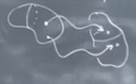
\includegraphics[width=15em]{16_01.png}

Gelinen noktaların hepsini beraber düşünürsek ortaya bir deforme olmuş
patates çıkacağını düşünebiliriz. Tabii başlangıcın illa patates olması
gerekmiyor, küre, herhangi bir şekil olabilir. Ben patates dedim çünkü üç
boyutlu genel bir kütlenin hayal edilmesini istedim. Neyse, iddia şu ki
Lorenz sistemi için akış sonrası gidilen deforme patatesin hacmi başlangıç
patatesinden küçüktür. Zaman geçtikçe hacim daha da küçülür. ``Yitirgen''
ile bunu kastediyoruz. Yitirgenlik birörnek (uniform) olmayabilir, bir
yönde az, diğer yönde daha fazla olabilir, fakat hacmin tamamında bir
azalma vardır.

Bu azalmayı görmek için kendimize şu soruyu soralım: hacim nasıl değişir?
Herhangi bir başlangıç hacmi $V(t)$'yi olsun, takip etmemiz gereken yegane
noktalar hacmi yüzeyinde olanlar, ve bu noktalardan başlayan gidiş yolları
sistemin vektör alanına göre akıyor olacaklar, o zaman bir süre sonra
$V(t + \Delta t)$ hacmi nedir? Bunu görmek için hacim için bir diferansiyel
denklem türeteceğiz. Hacim derken hacmi gösteren o tek sayıdan
bahsediyorum, tüm bölgenin şeklinden bahsetmiyorum.

Önce sezgisel argüman, notasyon 

$$ \underline{x} = (x,y,z)$$

$$ \underline{u} = \dot{\underline{x}} $$

olsun, yani $\underline{u}$ bu üç boyutlu faz uzayındaki hız. Bunlar şimdiye
kadar gördüğümüz şeyler, bir diferansiyel denklem olduğu zaman onun faz
uzayındaki vektör alanını düşünüyoruz, ki bu alan bize her noktada bir
vektör veriyor. Dikkat edelim, sıvı mekaniğiyle başladık şimdi ``hız''
dedik, ama bu hız sıvının akış hızı değil, faz uzayındaki soyut hızdan
bahsediyoruz.

Peki bu hızın hacmin yüzeyine dik olan bileşeni nedir? Eğer yüzeye dik bir
$\underline{n}$ vektörü düşünürsek, $\underline{u}$'nun o yöndeki bileşeni
$\underline{u} \cdot \underline{n}$ olur, biraz önceki eşitlik üzerinden
${\partial V}$ için (kısmi türev sembolü kullanıldı ama buradaki anlamı
``$V$ sınırı, onun dış çeperi'')

$$ 
\underline{u} \cdot \underline{n} = \dot{\underline{x}} \cdot \underline{n}
$$

${\partial V}$ yerine $S$ de kullanılabilir. 

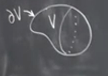
\includegraphics[width=10em]{16_02.png}

Sorumuz $\Delta t$ zamanı sonrası hacim nedir? Yani $V(t + \Delta t)$. 

Hacim değişimini zihinde canlandırmak için genel bağlamda genişlemeyi
modellemeye uğraşalım, $V$'nin dışında daha büyük bir patates hayal edelim
(küçülme de aynı mantık üzerinden hallediliyor) $V$ ona evrilmiş olsun,

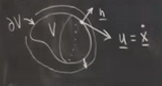
\includegraphics[width=15em]{16_03.png}

Resmin alt kısmındaki ok yüzeydeki bir noktanın nasıl genişlediğini
gösteriyor, ve diğer bir noktaya göre $\underline{n}$ gösterilmiş, ve hız
vektör alanının o noktadaki hali $\underline{u}$. Çizim bizi aldatmasın,
$\underline{u}$'yu teğet yapmaya uğraşmadım. 

Modelleme açısından şöyle düşünebiliriz, hacmin genişlemesi hızın yüzeydeki
normal bileşeni üzerindendir. O sebeple $\underline{u} \cdot \underline{n}$'e
odaklandım, çünkü hacim genişleme açısından bizi ilgilendiren en önemli
büyüklük bu. İddia şöyle, yeni $V(t + \Delta t)$, eski $V(t)$ artı hızın
normal yönde aştığı bir ufak bölgenin tüm mümkün bölgeler üzerinden entegre
edilmiş halidir.

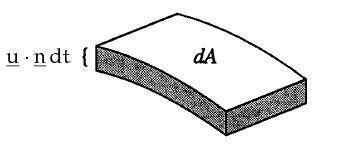
\includegraphics[width=15em]{16_04.png}

Üstte gösterilen ufak parçanın hacim değişimi yaklaşık olarak

$$ 
\Delta V \approx (\underline{u} \cdot \underline{n} \Delta t) \ud A
$$

O zaman, tüm bölgeler için

$$ 
V(t + \Delta t) \approx V(t) + 
\Delta t \iint\limits_{\partial V} \underline{u} \cdot \underline{n} \ud A
$$

Üstteki argüman tabii ki kulağa küpe / tahminsel / kestirme (heuristic) bir
argüman. Entegrale dikkat, bu bir yüzey entegrali. Eğer akı (flux) bazlı
düşünmek istersek üstteki hesap vektör alanı $\underline{u}$'nun dış akısı
olarak görülebilir.

Soru

Entegral niye yaklaşıksal, kesin değil? 

Cevap

$\Delta t$'yi limitte sıfıra götürdüğümüzde kesin olacak. 

Devam edelim, $V(t)$'yi sola geçirelim ve tüm formülü $\Delta t$'ye
bölelim.

$$ 
\lim _{\Delta t \to 0} \frac{ V(t + \Delta t) - V(t)}{\Delta t} = \dot{V(t)} =
\iint\limits_{\partial V} \underline{u} \cdot \underline{n} \ud A
$$

Nihai amacım bu formüldü, formül bana hacmin nasıl değiştiğini gösteriyor,
ki $\dot{V(t)}$ hacim değişimidir. Bu arada {\em Çok Değişkenli Calculus}
dersini almış olanlar için üstteki çift entegral tanıdık gelebilir,
formülün yapısı uzaklaşım (divergence) teorisini uygulamaya hazır, o çift
entegral $\underline{u}$'nun uzaklaşımının üçlü entegraline eşittir, yani

$$ 
\dot{V} = 
\iint\limits_{\partial V}  \underline{u} \cdot \underline{n} \ud A = 
\iiint \nabla \cdot \underline{u} \ud V
$$

Hacmin üç boyutlu faz uzayında herhangi bir vektör alanında nasıl
değiştiğini tarif eden formüller bunlar. Gerçi tahmin ederim ki boyut ne
olursa olsun formüller geçerlidir ama biz şimdilik üç ile kendimizi
sınırlayalım. 

Şimdi bu genel formülleri özelde Lorenz sistemine uygulayalım. Üçlü
entegralde bir $\underline{u}$'nun uzaklaşımından bahsediliyor. Lorenz
sisteminde $\underline{u}$'nun uzaklaşımı nedir? $\dot{V}$ formülünü tekrar
yazalım,

$$ 
\dot{V} = \iiint\limits_V \nabla \cdot \underline{u} \ud V
$$

Bu formülde hız $\underline{u} = (\dot{x}, \dot{y}, \dot{z})$, çünkü Lorenz
sisteminde faz uzayındaki hız budur değil mi? $\underline{u}$'nun
uzaklaşımı,

$$ 
\nabla \cdot \underline{u} = 
\frac{\partial \dot{x}}{\partial x} + 
\frac{\partial \dot{y}}{\partial y} + 
\frac{\partial \dot{z}}{\partial z} 
$$

Şimdi (6)'daki $\dot{x}, \dot{y}, \dot{z}$'leri bakarak üstteki türevleri
hesaplayalım ve formülde yerine koyalım,

$$ = -\sigma -1 - b$$

Hepsi negatif çıktı, ya da $-(\sigma+b+1)$. Bu hesap 1'den küçük olacaktır
çünkü $\sigma,b$'nin kesin pozitif oldugunu söylemiştik. Aslında çok iyi
bir sonuç bu, bir kere sabit. Bu sabit üçlü entegrali müthiş kolaylaştırır,
değil mi, çünkü $\nabla \cdot \underline{u}$ sabit, onun $\ud V$ üzerinden
entegrali hesaplanırken sabit entegral dışına çıkar, geri kalan sadece
$\ud V$'nin entegralidir, o da direk $V$ olur, yani hacmin ta kendisi. O
zaman

$$ \dot{V} = -(\sigma + b + 1) V$$

Bu sonuç hacimlerin üstel şekilde küçüldüğü anlamına gelir, çünkü

$$ V(t) = V(0) e^{-(\sigma + b + 1)}$$

Lorenz bunu gördü, üstteki sonuç direk onun makalesinden geliyor. Yani
elimizde bir başlangıç konum kütlesi var, ama bu kütle, ne olursa olsun,
sanki havasını kaybeden bir balon gibi küçülüyor, küçülüyor ve sonunda
sıfır hacme iniyor. Bu akılda tutulması gereken kuvvetli bir sonuç. Demek
ki tüm gidiş yolları sıfır hacimli bir limit kümesine gitmeye meyilli. Bu
küme bir tek nokta, bir çevrim olabilir, ya da bir ``garip çekici (strange
attractor)'' olabilir. Lorenz'in kendisi bu terimi kullanmamıştı, isim
sonradan verildi, ama Lorenz'in kullandığı terim de benim çok hoşuma
gidiyor, ``sonsuz yüzeyler kompleksi''. Bugün bu kavram fraktal olarak
biliniyor. Neyse, Lorenz bugünkü terimleri kullanmamış olsa da, sisteminde
çekicinin bir fraktal yüzey kümesi oldugunu görmüştü. O günlerde bilgisayar
grafiklemesi çok ileri değildi, Lorenz bir sanatçıya ne gördüğünü
çizdirmeye bile uğraştı, bu konuya sonra geleceğiz. Niye tek yüzey değil,
sonsuz kompleks yüzeyi?..

Kalan zamanımda bu limit kümesinin hangi şartlarda nokta oldugunu göstermek
istiyorum. Bu pek zor olmayan klasik bir hesap. 

Lorenz sistemindeki sabit noktaları bulalım. Cebire girmeyeyim, ama bir
tanesinin

$$ (x,y,z) = (0,0,0)$$

olduğu gösterilebilir. Bu sabit nokta her türlü parametre için geçerli. Bu
arada sistemin yapısını değiştiren parametre $\sigma,b,r$ demiştik ama
bunlardan sadece $r$ o amaçla kullanılıyor, Lorenz $\sigma=10,b=8/3$ ile
bunlardan iki tanesini sabitledi, sebepleri [2]'de bulunabilir. Yani klasik
parametre denen şey $r$. 

Orijin $(0,0,0)$ her $r$ için bir sabit nokta. Fakat orijin stabil değil,
su çarkı çerçevesinde bu dönüşün hiç olmadığı durum olurdu.

Bir diğer sabit nokta $x = y = \pm \sqrt{b(r-1)}$, $z=r-1$, eğer $r > 1$
işe, yani bu durumda $r$'nin yeterince büyük olması gerekiyor, aynen daha
önce şu çarkı durumunda gördüğümüz gibi, stabil dönüş için $r$'nin
yeterince büyük olması gerekiyordu. Dikkat edersek elimizde bir eksi ve
artı çift var, Lorenz onlara $C^+$ ve $C^-$ ismi vermiş, herhalde C
kullanmasının sebebi taşınım (convection) kelimesiyle alakalı, bu hareket
kalıbı kalıcı taşınım ima ediyor.

Ayrıca $r \to 1^+$ iken $C^+$ ve $C^-$'nin yani $x,y,z$'nin sıfıra
gittiğini görelim, yani orijinden bir geliş, ona gidiş var, burada bir tür
çatallaşma olmalı diye tahmin ediyoruz, ki bu hakikaten doğru, analize
devam edince $r=1$ noktasında bir tırmık çatallaşması oldugu
bulunabilir. Tırmık süperkritik tırmık, yani sabit noktalar doğduğunda
stabil durumdalar. 

Orijinin lokal stabilitesi nedir? Orijine yakında $x,y,z$ küçük olacaktır,
o zaman karesel terimleri yok sayabiliriz, ve lineerizasyon bize

$$ \dot{x} = \sigma (y-x)  $$

$$ \dot{y} = rx - y$$

$$ \dot{z} = -bz $$

verir. Görüldüğü gibi $z$ denklemi diğerlerinden bağlaşımsız hale geldi, ve $z$
üstel bir çürümeye sahip, yani $z(t) \to 0$ gidişi üstel hızda. Yanlız
dikkat bunları sistemin geneli için söylemiyorum, bu lineerizasyon,
söylenenler orijin etrafında geçerli. 

O zaman $z$'ler çürüyor, geriye elimizde $x,y$ bağlamında iki boyutlu ufak
bir sistem kalıyor. Bu sistemi ayrı bir şekilde irdeleyebiliriz, matris
formunda 

$$ 
\left[\begin{array}{r} \dot{x} \\ \dot{y} \end{array}\right] =
\left[\begin{array}{rr}
-\sigma & \sigma \\ r & -1 \end{array}\right]
\left[\begin{array}{r} x \\ y \end{array}\right]
$$

Daha önce öğrendiğimiz iki boyutlu tekniklerle bunun $x,y$ dinamiği için
anlamını analiz edebiliriz. İz $\tau = -\sigma - 1 < 0$, determinant
$\Delta = \sigma(1-r)$. $r > 1$ ise orijinde bir eğer (saddle) noktası
var çünkü determinant negatif. Fakat burada ilginç bir durum var, bu eğer
noktası değişik bir tür eğer. Üç boyuttayız, iki boyutta geliş bir boyutta
gidiş var. 

Devam edelim 

$$\tau^2 - 4\Delta = (\sigma+1)^2 - 4\sigma(1-r)$$

$$ = (\sigma-1)^2 + 4\sigma r > 0$$

Yani $\tau^2 - 4\Delta$ her zaman pozitif, eğer $r < 1$ ise o zaman
$\Delta$ pozitif, $\tau^2 - 4\Delta$ da pozitif, $\tau$ negatif oldugu için
her $x,y,z$ yönünde elimizde bir stabil düğüm (node) var.

Kaynaklar

[1] Strogatz, {\em Video}, \url{https://www.youtube.com/watch?v=7iNCfNBEJHo}

[2] Lorenz, {\em Deterministic Nonperiodic Flow}, \url{http://eaps4.mit.edu/research/Lorenz/Deterministic_63.pdf}

\end{document}





